\documentclass{article}

% Source file of ndsu-thesis-2022 class documentation (ndsu-thesis-2022-documentation.tex). The images used (3 total) are stored in /figures/ subfolder. 

%--------------------------------------------------------------
\usepackage[nonewpage]{imakeidx}
\makeindex[intoc, columnseprule, columns=3, columnsep = 2.5cm]
\usepackage[top=1in,bottom=1.2in,left=1in,right=1in,letterpaper]{geometry}
\usepackage{verbatim}
\usepackage{tocloft}
\usepackage{xparse}
\usepackage{xspace}
\usepackage{xcolor}
\usepackage{booktabs}
\usepackage{graphicx}
\usepackage{siunitx}
\usepackage{soul}
\usepackage[colorinlistoftodos,prependcaption,textsize=scriptsize]{todonotes}
\usepackage{tikz}
\usepackage{multicol}
\usepackage{tabularray}
\usepackage{caption}
\usepackage{enumitem}
\usepackage[hidelinks]{hyperref}

%--------------------------------------------------------------
%--------------------------------------------------------------
\graphicspath{{./figures/}}

\newcommand\cmd[1]{\textbackslash\texttt{#1}}
\newcommand\tb\textbackslash
\definecolor{newtext}{rgb}{0.1,0.6,0.1}
\newcommand\nt[1]{\textcolor{newtext}{#1}\xspace} % annotation command
\newcommand\dt[1]{\textcolor{red}{\st{#1}}\xspace} % annotation command
\newcommand\rt[2]{{\textcolor{red}{\st{#1}}}{\textcolor{newtext}{#2}}\xspace} % annotation command
\newcommand\notes[1]{\vspace{2ex}\todo[color=green!35, inline]{#1}} % todo notes
\newcommand\ix[1]{#1\index{#1}} % shortcut for index - #1 twice to retain text
\newcommand\ixt[1]{#1\index{\texttt{#1}}} % shortcut for index - #1 twice to retain text
\newcommand\ixl[1]{#1\lowercase{\index{#1}}} % shortcut for index
\newcommand\ixm[2]{#2\index{#1!#2}} % shortcut for index - muti level
\newcommand\ixmt[2]{\index{#1!\texttt{#2}}} % shortcut for index - mutilevel
\setlength{\parindent}{0.3in}

\newcommand\ccmd[1]{ % shortcut for centered commands
\begin{center}
\begin{tabular}{l}
#1
\end{tabular}
\end{center}
}

%\setlength{\columnsep}{3cm}

%--------------------------------------------------------------
%--------------------------------------------------------------
\title{\vspace{-1.5cm}Using the \texttt{ndsu-thesis-2022} \LaTeX\/ class --- Documentation}
\author{Aaron Feickert$\,^{a}$, Jonathan Totushek$\,^{a}$, and C. Igathinathane$\,^{b,\,*}$ \\ *\,Maintainer, Bug Reports and Enquires:  Igathinathane Cannayen (\texttt{i.cannayen@ndsu.edu})\\ {\small Github: \url{https://github.com/CIgathi/NDSU-Thesis-Class.git}}
}
\date{{\small $^{a}$\emph{Department of Mathematics, NDSU} \\ $^{b}$\emph{Department of Agricultural and Biosystems Engineering, NDSU}\\[2ex]}
24 October 2022}

%--------------------------------------------------------------
%--------------------------------------------------------------
%--------------------------------------------------------------
\begin{document}
\maketitle

\hrule
\begin{multicols}{2}
\scriptsize
\tableofcontents
\end{multicols}
\hrule

%--------------------------------------------------------------
%--------------------------------------------------------------
\section{Introductions}
The \texttt{ndsu-thesis-2022} \LaTeX\ is an updated version of the previous \texttt{ndsu-thesis} \ix{class} file. This class generates disquisitions intended to comply with the disquisition requirements of the North Dakota State University (NDSU) Graduate School. This class is not officially endorsed by NDSU or the NDSU Graduate School, but efforts are underway toward that goal. It should be noted that several theses and dissertations were made and got approved by the Graduate School using the NDSU \LaTeX\ thesis class in the past. Since disquisition requirements are subject to change at any time, the user is advised that the most current disquisition style policies supersede this class. However, following the Graduate School approved template and collected experience from several previously approved dissertations, this \LaTeX\ class was coded to incorporate the various required features and lessons learned, while preparing theses/dissertations using the previous class, in developing this version of the class. To ensure compliance with all NDSU Graduate School requirements, the user is encouraged to consult the NDSU Graduate School webpage and the links provided for detailed requirements and guidance on disquisition formatting guidelines, templates, section formatting, and examples (\url{https://www.ndsu.edu/gradschool/current_students/graduation/theses_dissertations_papers/disquisition_formatting}).

The bundled \ix{template} or the \ix{example} given (Section~\ref{example}) can be used as an easy starting point for using the class. Modification of the class file's code may result in unexpected behavior and is at the user's own risk. We recommend including additional packages and commands in the source file (*.tex) itself for the desired customization as required by the departments and the users. 

%--------------------------------------------------------------
%--------------------------------------------------------------
\section{Using and installing \LaTeX\  --- online and desktop environments} \index{online editor} \index{standalone editor}
Several online (e.g., Overleaf, Kile LaTeX Editor, Authorea, Papeeria, and so on) and standalone desktop versions (e.g., TeXMaker, TeXWorks, TexShop, TeXStudio, and so on) of \LaTeX\ editors are available. Online editors are ``ready-to-go,'' with several templates, tutorials, and help documentation, where the user need not install the software but require an internet connection. The desktop version requires software installation and updating (not very frequent). Resources (text and video instructions) are available on both how to use the online editor and install the \LaTeX\ desktop version of users' choice. As \LaTeX\ is open source, most of these editors are free.

%--------------------------------------------------------------
%--------------------------------------------------------------
\section{Documentclass Options}
These are the \ix{options} passed to the \ix{documentclass} command while calling the class. These options essentially affect the whole document and a \ix{default behavior} (no options specified, shown below) was also valid.
\ccmd{\cmd{documentclass\{ndsu-thesis-2022\}}}
The above default behavior with no \texttt{[options]} specified produces a Ph.D. dissertation in 12 pt font size with auto-numbered heading and justified text in computer modern font. However the command:\vspace{-2ex}\ccmd{\cmd{documentclass[ms-thesis,11pt,nonumber,nojustify,draft,showframe,times]\{ndsu-thesis-2022\}}} produces an M.S thesis in 11 pt font size unjustified paragraphs text with unnumbered heading in draft mode in Times Roman font and shows the frame using the set margins. The order in which these options are passed does not matter. The various options are briefly discussed subsequently.

%--------------------------------------------------------------
\subsection{Disquisition degree and type}
\label{degtype}
By default, this class assumes the document is a Ph.D. dissertation. Providing a degree option will accommodate other available degree and disquisition types (Table~\ref{degree}):

\begin{table}[h!]
\centering
\caption{Options for degree and disquisition types}
\vspace{-1.5ex}
\begin{tabular}{lll}
\toprule
Option & Degree & Disquisition type \\
\midrule
\texttt{[\ixm{degree}{phd}]} & Ph.D. & Dissertation \\
\texttt{[\ixm{degree}{ms-thesis}]} & M.S. & Thesis \\
\texttt{[\ixm{degree}{ms-paper}]} & M.S. & Paper \\
\texttt{[\ixm{degree}{ma-thesis}]} & M.A. & Thesis \\
\texttt{[\ixm{degree}{ma-paper}]} & M.A. & Paper\\
\bottomrule
\end{tabular}
\label{degree}
\end{table}

%--------------------------------------------------------------
\subsection{Font size}
The general \ix{font sizes} used with thesis are 10, 11, and 12 points and they vary with the selected font. The available options (any of these used) are:
\ccmd{\cmd{documentclass[10pt (or) 11pt (or) 12pt]\{ndsu-thesis-2022\}}}
The default was set as {\tt{12pt}}.

%--------------------------------------------------------------
\subsection{Auto-numbered, chapter-numbered, and unnumbered styles}
The three possible NDSU thesis styles with options included are: (i) Auto-numbered [default option] --- where chapters, sections, subsections, and so on will be numbered; (ii) Chapter-numbered [\ix{chapternumber}] --- where only chapters are numbered, while sections, subsections, and so on will not be numbered; and (iii) Unnumbered [\ix{nonumber}] --- where all headings such as chapters, sections, subsections, and so on will not be numbered.

As the default is the numbered style, the chapter-numbered and unnumbered styles were produced by the ``chapternumber'' and ``nonumber'' options respectively as: \ccmd{\cmd{\ix{documentclass}[chapternumber (or) nonumber]\{ndsu-thesis-2022\}}} The default was the ``Auto-numbered'' style. These options will have their specific effect on the numbering scheme of the tables and figures.

%--------------------------------------------------------------
\subsection{Paragraph text justification}
Based on their preference students can follow \ix{fully-justified} (with hyphenated words and word wrapping) or unjustified (no word breaking but right margin ragged, aka left-justified). As the default is justified, the \ix{left-justified} passages were produced by the \texttt{[\ix{nojustify}]} option. For justified style, nothing needs to be specified. NDSU approves both styles.

%--------------------------------------------------------------
\subsection{Draft and display \ix{document frames}}
You can use the \texttt{[\ix{draft}]} option to place the disquisition into draft mode. In this mode, \ix{margin overflows} are marked with a heavy black box to draw your attention to them; additionally, images are replaced by a \ix{placeholder} (see Fig.~\ref{fig:frame}). If you import other packages in your disquisition, they may also change their behavior when in draft mode.

\begin{figure}[h!]
\centering
\vspace{-0.8ex}
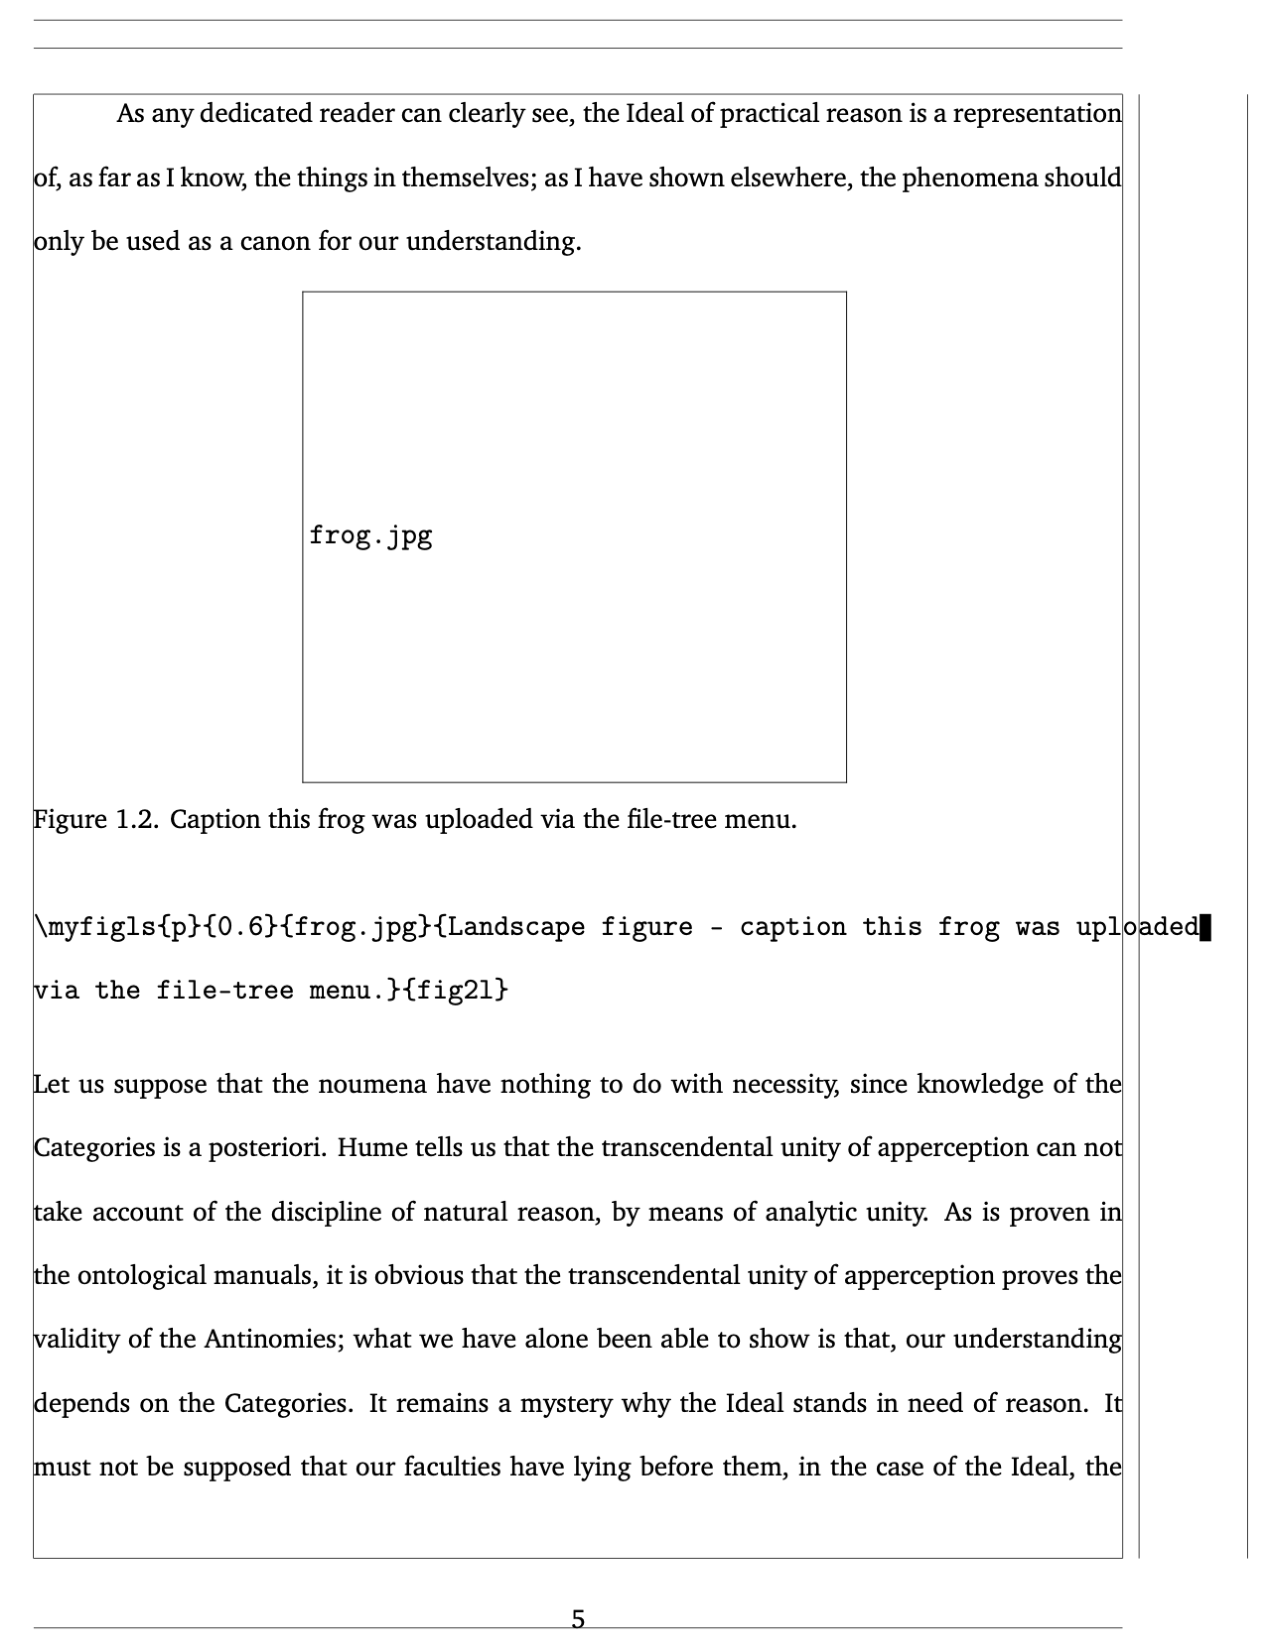
\includegraphics[width=0.525\textwidth]{fig-draftmargin.pdf}
 \caption{Use of \texttt{draft} and \texttt{showframe} options in \texttt{documentclass} producing image placeholder for quicker processing, document frames, and margin overflows.}
\label{fig:frame}
\end{figure}

\indent The \texttt{[\ix{showframe}]} option (based on \texttt{\ix{geometry}} package) produces a frame around the text area which can be used to check how the text aligns with the margins (left, right, top, and bottom; see figure above). The illustration alongside displays the result of these options showing the overflowing text, bottom \ix{margin frame}, right margin frame, margin notes frames, and the \ix{overflow} heavy black box. The default behavior is these options were inactive.

%--------------------------------------------------------------
\subsection{Fonts}\index{font}
The following \ix{font options} \texttt{[\ixm{font}{bookman}, \ixm{font}{charter}, \ixm{font}{gentium}, \ixm{font}{kpfonts}, \ixm{font}{libertine}, \ixm{font}{mathdesign}, \ixm{font}{mathptmx}, \ixm{font}{newcent}, \ixm{font}{palatino}, \ixm{font}{tgtermes}, \ixm{font}{times}, \ixm{font}{tgbonum}, \ixm{font}{tgpagella}, \ixm{font}{tgschola}, \ixm{font}{utopia}, \ixm{font}{zlmtt}]} are compatible with the class, and anyone can be used. The default was \LaTeX\ computer modern font. Users are urged to check the NDSU approved fonts and select that resembles them and use them with appropriate font sizes.

%--------------------------------------------------------------
\subsection{Advanced options}\label{adop}
Although not required for simple work, a few class options were made available to further automate the dissertation writing. The first option is \texttt{[\ix{chaptersbib}]}. This is intended to produce individual chapter bibliography and should only be used with Bib\LaTeX\/ and BibTeX will not support chapters bibliography --- based on this class. This option works with chapters processed as ``\ix{subfiles},'' where those chapters can be individually compiled and output generated.

The second option is \texttt{[\ix{subfileref}]}. Subfiles, usually individual chapters, can be processed individually following the same style of the whole document. The information in the preamble of the main dissertation document (that pulls in and assembles all the chapters of the dissertation in individual files) was again derived and used as the preamble of the subfile. The required package ``\texttt{subfiles}''  was included in the class. For each chapter to be standalone, like a paper, the chapter should have the relevant bibliography as the last unnumbered section/chapter, and using this option in the main document will accomplish this. This option work with both Bib\LaTeX\/ and \ix{BibTeX}. The whole dissertation processing, obtaining contents from these individual subfiles, with intended combined bibliography chapter, should not also produce the individual chapters bibliography, therefore this option should not be used. Refer to the additional example in the class bundle that shows the necessary codes in the main and chapter files.

The following table shows the various outcomes given the options (Table~\ref{chapoption}):
\vspace{-1ex}
\begin{table}[h!]
\centering
\caption{Options for degree and disquisition types}
\vspace{-1.5ex}
\begin{tabular}{lp{4in}}
\toprule
Option & Outcomes \\
\midrule
\texttt{[\ix{chaptersbib}]} only & Dissertation with individual chapters bibliography. Works with Bib\LaTeX\/ only. \\
\texttt{[subfileref]} only & For individual chapter processing bibliography. Works with both Bib\LaTeX\/ and BibTeX.\\
\texttt{[]} none --- default & Dissertation with combined bibliography as unnumbered chapter.  \\
\texttt{[chaptersbib,subfileref]} both & \emph{Don't use}. Possible redundant bibliographies. Requires Bib\LaTeX\/. \\
\bottomrule
\end{tabular}
\label{chapoption}
\end{table}

%--------------------------------------------------------------
%--------------------------------------------------------------
\section{Preamble Information}

%--------------------------------------------------------------
\subsection{General information - packages and shortcuts}
If your disquisition requires the use of additional \LaTeX\ packages, macro files, or other commands, include them in the preamble. Packages such as \texttt{\ix{natbib}} (author-year and number style citations) or other competent reference handling packages and their options can be loaded. Similarly, mathematical \ix{theorem environment}-related commands (theorem, corollary, lemma) through \cmd{newtheorem} of \texttt{amsthm} package, \texttt{caption} package setups through \cmd{captionsetup[\emph{type}]\{\emph{options}\}}, where \emph{\texttt{type}} = table, figure, or subfigure, and other shortcuts for repetitive longer commands or text can be defined in the preamble. As these are specific to the users and the requirements vary with the users of different specializations, these were not included in the class. Therefore suitable packages, commands, and shortcuts can be defined by the users.

%--------------------------------------------------------------
\subsection{Dissertation front pages}
Before issuing the \cmd{begin\{document\}} command, several pieces of preamble information are available.

%--------------------------------------------------------------
\subsubsection{Title}
Include the \ix{title} of the disquisition using the \cmd{title\{\ldots\}} command. This is required.

%--------------------------------------------------------------
\subsubsection{Author}
Include the full name of the disquisition \ix{author} using the \cmd{author\{\ldots\}} command. This is required.

%--------------------------------------------------------------
\subsubsection{Major \ix{department}/\ix{program} choice}
Specify whether it is ``Department'' or ``Program'' that is applicable using the \cmd{progdeptchoice\{\ldots\}} command. This will produce ultimately ``Major Department:'' or ``Major Program:'' based on the input choice. This is required.

%--------------------------------------------------------------
\subsubsection{Department or program}
Include the name of the major \ix{department} or \ix{program} using the \cmd{department\{\ldots\}} command. This is required.

%--------------------------------------------------------------
\subsubsection{Degree option}
If the major department or program has a \ix{degree} option, indicate this using the \cmd{degreeoption\{\ldots\}} command. This is optional.

%--------------------------------------------------------------
\subsubsection{Date}
Include the date of the final examination using the \cmd{\ix{date}\{\ldots\}} command. The accepted format of this date is \textit{month year} as: \cmd{date\{October 2022\}}. This is required.

%--------------------------------------------------------------
\subsubsection{Examining committee}
Include the Chair (or Co-Chairs) and members of the examining committee using separate commands. The \cmd{\ix{cchair}\{\ldots\}} command is used to indicate the committee Chair. Use \cmd{\ix{cochairZ}\{\ldots\}} to indicate any committee Co-Chair members, where \texttt{Z} is \texttt{a} or \texttt{b}. This class does not support more than two Co-Chairs and four Committee Members. Use the \cmd{cmemberX\{\ldots\}} to indicate other committee members, where \texttt{X} is \texttt{a}, \texttt{b}, \texttt{c}, or \texttt{d}. Use only as many of these commands as needed to list all committee members.

%--------------------------------------------------------------
\subsubsection{Approval information}
Use the \cmd{approvaldate\{\ldots\}} command to include the full date of \ix{disquisition approval} (i.e. month/date/year). This date is generally the date the thesis was approved by the Department Chair following the defense after the approval (usually electronically) of all committee members. Use \cmd{approver\{\ldots\}} to include the Department Chair who approved the disquisition. Both commands are required.

%--------------------------------------------------------------
\subsection{Dissertation front matter}

\subsubsection{Abstract}
Use the \cmd{\ix{abstract}\{\ldots\}} command to include the disquisition abstract. Abstracts for doctoral dissertations must use 350 words or less. Abstracts for master's papers or master's theses must use 150 words or less. This is required.

%--------------------------------------------------------------
\subsubsection{Acknowledgements}
If the disquisition includes \ix{acknowledgements}, include them using the \cmd{acknowledgements\{\ldots\}} command. This is optional.

%--------------------------------------------------------------
\subsubsection{Dedication}
If the disquisition includes a dedication, include it using the \cmd{\ix{dedication}\{\ldots\}} command. This is optional.

%--------------------------------------------------------------
\subsubsection{Preface}
If the disquisition includes a \ix{preface}, include it using the \cmd{preface\{\ldots\}} command. This is optional. The NDSU guidelines state:
\begin{quote}
``\emph{The Preface can provide an autobiographical account of how the disquisition came to be or include a significant quote that drove your research. Follow the General Requirements for font, spacing, and page numbers for prefatory materials.}''
\end{quote}

%--------------------------------------------------------------
%--------------------------------------------------------------
\section{Automatic Components}
Several \ix{automatic components} will be generated, as a part of the front matter, based on the source code of the dissertation and are briefly described. Based on the department, requirement, and style of the thesis some of the items such as, lists of abbreviations, symbols, and appendix tables and figures (Secs.~\ref{sloa}--\ref{sloat}) may be dropped from the coding.

%--------------------------------------------------------------
\subsection{Table of contents}
The \ix{table of contents} (\ix{TOC}) gets automatically generated with entries up to three levels sections (\cmd{my...heading}, \cmd{section}, and \cmd{subsection}). The dissertation may have further levels of sections but they are not shown in the TOC.

%--------------------------------------------------------------
\subsection{List of \ix{table}s and \ix{figure}s}
The \ix{list of tables} (\ix{LOT}) and \ix{list of figures} (\ix{LOF}) will be generated based on the table and figure full captions in the \texttt{table} and \texttt{figure} environments. New commands for handling figures such as \cmd{myfig\{1+5 arguments\}}, and \cmd{myfigls\{1+5 arguments\}} with their own \texttt{[optional]} argument to adjust the position of the caption with respect to figure element were defined.

%--------------------------------------------------------------
\subsection{List of abbreviations}\label{sloa}
The collection of abbreviations used in the dissertation can be made in to a \ix{list of abbreviations} (\ix{LOA}) using the \cmd{listofabbreviations\{\ldots\} command. This collection should be alphabetized before coding. This will be a two-column tabular entry. A two entry example of LOA code and the output are shown below:
\begin{tabbing}
xxxx\= \kill
\> \cmd{listofabbreviations\{} \\
\> \texttt{AC \& Alternating current\tb\tb} \\
\> \texttt{NDSU \& North Dakota State University\}}
\end{tabbing}
}
{\vspace*{-0.65in}\hspace*{3.7in}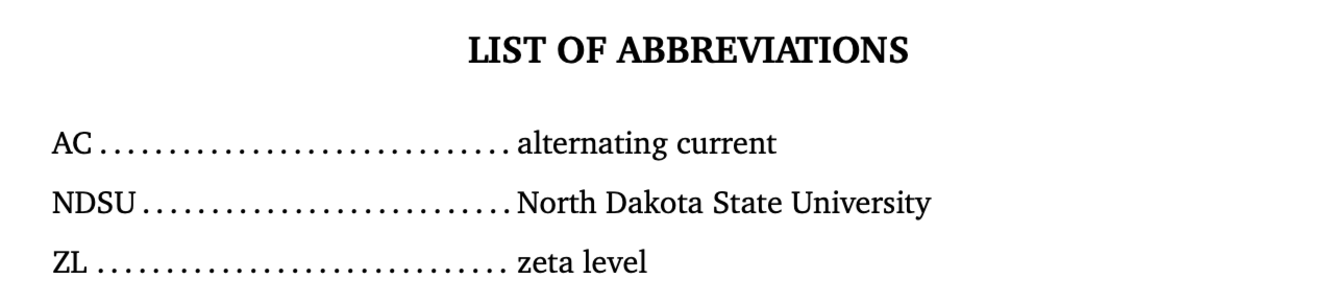
\includegraphics[width=0.45\textwidth]{fig-LOA.pdf}}

%--------------------------------------------------------------
\subsection{List of symbols}\label{slos}
The collection of all technical symbols used in the dissertation, usually coded in ``math'' mode, can be made into a \ix{list of symbols} (\ix{LOS}) using the \cmd{listofsymbols\{\ldots\}} command. This collection should be alphabetized before coding and math mode should be used as required. This will be a two-column tabular entry. A three-entry example of LOS also using the \texttt{siunitx} package and the output are shown below:
\begin{tabbing}
xxxx\= \kill
\> \cmd{listofsymbols\{} \\
\> \texttt{\$A\$ \& Area (\tb si\{\tb m\tb squared\}) \tb \tb} \\
\> \texttt{\$c\$ \& Speed of light (\tb SI\{299.792\}\{\tb km\tb per\tb s\})\tb \tb} \\
\> \texttt{\$R\^{}2\$ \& Coefficient of determination}\}
\end{tabbing}
{\vspace*{-0.8in}\hspace*{3.95in}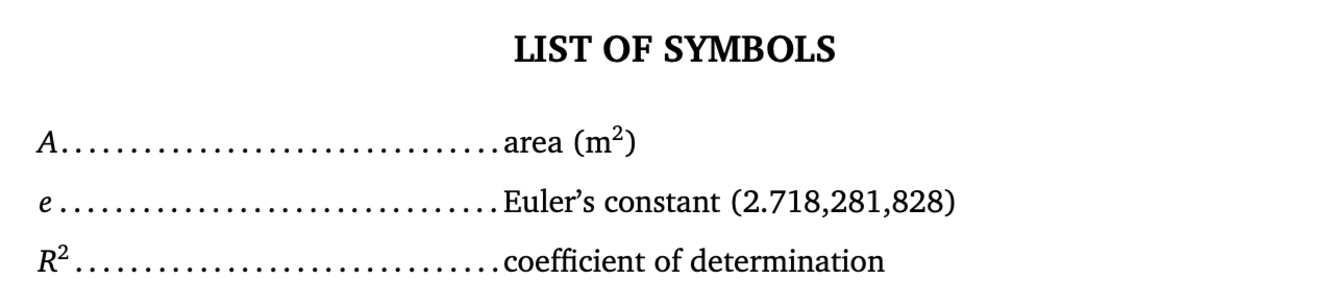
\includegraphics[width=0.5\textwidth]{fig-LOS.pdf}}

%--------------------------------------------------------------
\subsection{List of appendix tables and figures}\label{sloat}
The \ix{list of appendix tables} (\ix{LOAT}) and \ix{list of appendix figures} (\ix{LOAF}) will be generated based on the appendix table and figure full captions in the \texttt{appendixtable} and \texttt{appendixfigure} environments. New commands such as \cmd{myfigap\{5 arguments\}} and \cmd{myfigapls\{5 arguments\}} plus one \texttt{[optional]} argument for adjusting the caption placement for regular and landscape figures were defined.

The \cmd{\ix{closeappendices}} command should be issued at the end of the last appendix, which ensures the automatic creation of the LOAT and LOAF when the appendices had tables and figures. If the appendices had only tables or only figures then the commands \cmd{closeappendixtables} or \cmd{closeappendixfigures} should be used to avoid blank entries.

%--------------------------------------------------------------
%--------------------------------------------------------------
\section{Beginning the Document}
After including the necessary preamble information, use \cmd{begin\{document\}} to start the \ix{document}. This command automatically generates the necessary cover pages and other automatic components. The usual \cmd{\ix{maketitle}} command should not be used, as it was already issued in the class.

%--------------------------------------------------------------
%--------------------------------------------------------------
\section{Headings}\label{heading}\index{heading}
Major headings (e.g. chapters) are issued using the \cmd{myheading\{\ldots\}} command. This command supersedes the usual \cmd{\ix{chapter}} command, which should not be used. The following shows the hierarchy of headings:
\ccmd{
\cmd{\ixm{heading}{myheading}\{\ldots\}} \hspace{0.6in} Produces all-caps chapter headings automatically - 0th level\\
\cmd{\ixm{heading}{mypaperheading}\{\}\{\}\{\}} \hspace{2.9ex} Produces all-caps paper chapter headings with footnote - 0th level\\
\cmd{\ixm{heading}{section}\{\ldots\}}  \hspace{0.74in} Produces centered, bold headings (use title case) - 1st level\\
\cmd{\ixm{heading}{subsection}\{\ldots\}} \hspace{0.52in} Produces left-aligned, bold headings (use title case) - 2nd level\\
\cmd{\ixm{heading}{subsubsection}\{\ldots\}}\hspace{0.35in}  Produces left-aligned, bold, italic headings (use sentence case) - 3rd level\\
\cmd{\ixm{heading}{paragraph}\{\ldots\}}\hspace{0.64in}  Produces left-aligned, italic headings (use sentence case) - 4th level
}

Each \cmd{myheading\{\ldots\}} or \cmd{mypaperheading\{3 args\}} command starts a new page and entry in the table of contents.  The regular chapter command is simple and takes one argument which is the title of the chapter as \cmd{myheading\{title\}}. The paper-styled chapter takes three arguments that address the title and footnote as
 \cmd{mypaperheading\{title\}\{footnotemark\}\{footnotetext\}}.  The \texttt{title} is common to both styles and will be rendered as all-caps irrespective of the input.  The \texttt{footnotemark} usually be an asterisk (*),  but can be any valid footnote mark including math symbols.  The footnote mark will be used in the footnote text but will not feature in the TOC.  The footnote text will be rendered as a footnote on the same page and automatically uses the input footnote mark.  

In general,  the paper-styled chapter requires an ``Abstract'' section (title coded as a section),  while the regular chapter does not.  The class is coded to produce a consistent space between the title and the text (or section) below the title; however when necessary \cmd{vspace\{+ve or -ve\}} can be issued before the plain introductory text or section command to adjust this vertical space.  

Instances of \cmd{subsubsection\{\ldots\}} and \cmd{paragraph\{\ldots\}} do not appear in the TOC, though they are included in the document.  Other than the chapter headings,  the rest of the item headings should be coded by the user manually with appropriate capitalization (title and sentence cases).

%--------------------------------------------------------------
%--------------------------------------------------------------
\section{Dummy Text and Images}\index{dummy text} \index{dummy images}
Users will be curious to see what their thesis/dissertation will look like quickly without using the actual texts and figures. The class comes loaded with necessary packages such as \texttt{kantlipsum}\index{kantlipsum} (for dummy text --- philosophical prose paragraphs in English) and \texttt{mwe}\index{mwe} (``minimal working examples'' for dummy images). These will help visualize the whole document (fonts, spacings, and layout) with minimal effort, and this is a common practice among typesetters to use such dummy text and images. Commands from these packages are used in the thesis example (Sec.~\ref{example}).

Commands like \cmd{kant[1]} or \cmd{kant[4-8]} will produce single or multiple dummy text paragraphs. Similarly, dummy images included in the \texttt{mwe} package can be accessed using their specific names and can be used as the image argument in the \cmd{includegraphics} command, which means that the user need not use their images. Some of the commonly used examples images are: \texttt{example-image}, \texttt{example-image-a}, \texttt{example-image-b}, \texttt{example-image-c}, \texttt{example-image-16x10}, \texttt{example-image-golden}, \texttt{example-image-pl} \texttt{ain}, \texttt{example-image-duck}, \texttt{example-image-empty}, and \texttt{example-} \texttt{grid-100x100pt}\index{example images}. Refer to the documentation of these packages for further information.

%--------------------------------------------------------------
%--------------------------------------------------------------
\section{Tables and Figures}
\subsection{Tables}
Different kinds of tables, such as simple table without caption (\texttt{\ixm{table}{tabular}}), table with \ixm{table}{caption} (\texttt{table}), table with \ixm{table}{footnote} (\texttt{\ixm{table}{threeparttable}}), table spanning entire text width (\texttt{\ixm{table}{tblr}}), table spanning multiple pages (\texttt{\ixm{table}{longtable}}), and table in \ixm{table}{landscape} page (\texttt{\ixm{table}{pdflscape}}) can be coded following the documentation of respective packages, and no shortcuts were defined as they were not practical. Using \texttt{\ixm{table}{booktabs}} package professional quality tables (Sec.~\ref{degtype}) can be created.

%--------------------------------------------------------------
\subsubsection{Full-width tables --- \texttt{tblr} environment from \texttt{tabularray} package}\index{table!full-width}
Full-width tables are suggested for NDSU theses/dissertations. A quick and efficient method of creating tables that automatically span the entire textwidth is the use of \texttt{tblr} (short for \texttt{top-bottom-left-right} or \texttt{tabularray}) environment instead of the usual \texttt{tabular} inside the \texttt{table} environment. The \texttt{tblr} environment (from \texttt{tabularray} package) uses a special column justification code X (default \& options). This X code allots fixed column width based on the number of columns specified (default) and customizes individual columns' proportional width using coefficients with options. The \texttt{tblr} also takes the usual \texttt{l, c, r,} and \texttt{p} justification codes as well as the commands of \texttt{booktab} in the usual manner. The \texttt{tblr} environment is from the latest package and has several special features such as, specifying exclusive \texttt{math} mode column (no \$ symbols required for individual items); SI~units features; colored rows, cells, and lines; and so on (See \texttt{tabularray} package documentation).

%--------------------------------------------------------------
\subsubsection{Full-width tables --- manual method} \index{table!full-width}
However, for the best control of tables, especially with more columns, a combination of \cmd{resizebox} (resizing the entire table - mostly for scaling down) and \cmd{tabcolsep} (maintaining the column separation space) works the best. Thus, the command \cmd{\ixm{table}{resizebox}\{\cmd{\ixm{table}{columnwidth}}\}}\{!\} makes the table to span the entire text width of the page. This will expand or shrink the contents of the table to fit the entire width. It should be fine with the fonts shrink to fit the width, but will not be when the fonts enlarge (especially when the table is small and has only a few columns). In such situations, the space between the columns can be adjusted using the \cmd{\ixm{table}{tabcolsep}\{\ldots\}} command, where increased spacing reduces the font size and \emph{vice versa}. Thus, by using these commands (including \texttt{tblr}) in combination the tables and the font size can be scaled down to fit the page with the proper font size.

%--------------------------------------------------------------
\subsubsection{Table row spacing and fonts}
The row spacing can be adjusted, if desired, using \cmd{renewcommand}\{\cmd{\ixm{table}{arraystretch}}\}\{\ldots\} inside the table environment. For example, a value of 1.75 for the arraystretch will be similar to the double line spacing; and without this command, the row spacing will be single line spacing. Table footnotes can be added through \texttt{\ixm{table}{tablenotes}} environment placed inside \texttt{table} environment after the \texttt{tabular} and \texttt{resize} blocks. The font size can be altered by selecting the standard sizes (e.g., \cmd{footnotesize}, \cmd{small}) within the \texttt{tablenotes} environment.

%--------------------------------------------------------------
\subsubsection{Landscape tables}
When a table has more columns of information, the most common solution is the landscape orientation which is achieved through \texttt{\ixm{table}{landscape}} environment by enclosing the \texttt{table} codes (which may contain other elements) inside \texttt{landscape} environment block (between \cmd{begin\{landscape\}} and \cmd{end\{landscape\}}). With landscape usually the placement option will be [p] and the whole width should be set around 1.32 times the \cmd{\ix{columnwidth}}, or adjusted suitably to leave acceptable margins all around.

%--------------------------------------------------------------
\subsection{Figures}\label{figs}
It should be noted that the manual coding of figures using ``\texttt{figure}'' environment with \cmd{\ixm{figure}{includegraphics}\{\ldots\}} \ixm{figure}{centering}, \ixm{figure}{resize}, \ixm{figure}{caption} and \ixm{figure}{label}s is the direct approach.

%--------------------------------------------------------------
\subsubsection{Shortcuts for figures --- direct and optional}\label{figureshortcut}
However, for convenience, a set of single command shortcuts, with five arguments plus one optional argument are defined. These commands specify (1) [optional] vertical placement of the caption (moving it up and down with respect to the bottom of the figure, especially for images with excessive or too less whitespace), (2) placement, (3) size factor, (4) input file, (5) caption, and (6) label were defined to produce figures (regular and landscape). The default caption's \texttt{aboveskip} is \verb|0ex|, and this value can be changed using the optional argument. Following are the examples of figure shortcuts for regular and landscape figures without and with the optional argument. These shortcuts are automatically included in the LOF and LOT that appear after the TOC. \index{figure!myfig} \index{figure!myfigls}

\begin{flushleft}
\hspace{0.2cm}
\begin{minipage}{0ex}
\begin{verbatim}
 \myfig{ht}{0.7}{image1.jpg}{Caption for this regular figure}{fig:1}
 \myfig[1.5ex]{ht}{0.7}{image1o.jpg}{Figure caption with placement option}{fig:1o}

 \myfigls{p}{1.32}{image2.pdf}{Caption for this landscape figure}{fig:2ls}
 \myfigls[2ex]{p}{1.31}{image3.pdf}{Landscape figure caption with placement option}{fig:3ls}
\end{verbatim}
\end{minipage}
\end{flushleft}

%------------------------
Sometimes, excessive spaces were observed above and below the figures and tables (floating elements) as well as equations with respect to the text around. The use of vertical spacing (+ve or -ve; e.g., \cmd{vspace\{4pt\}} and \cmd{vspace\{-6pt\}}) around the floating elements can help in the adjustment of their placements. \index{figure!placement} The \ix{vertical spacing} commands can be issued before and after these environments (as required) to fix the spacing. Coding tables and figures will automatically create the LOT and LOF. A similar approach can be used for appendix figures (Sec.~\ref{apfigtab}).

%--------------------------------------------------------------
\subsection{Captions}
Because of the way spacing is handled, \ix{caption}s in \texttt{table} environments must appear at the top of the table, while captions in \texttt{figure} environments must appear at the bottom of the figure. If you use both \cmd{caption} and \cmd{label} commands in these environments, the \cmd{caption} command must come before the \cmd{label} command to ensure the environment is numbered correctly. The captions are coded in such a way that shorter ones are centered and longer ones are left-justified; however, as default the table captions are left-justified and can be changed,  as outlined subsequently, to fit the requirement.  The style of the caption can be basic or specific to the department, usually following the parent technical society's leading journal. The style of labeling (e.g., regular \emph{vs} bold \emph{vs} italic, naming: Fig. \emph{vs} fig. \emph{vs} Figure, etc.) can also be adopted from the leading journal. The various options available for caption using the \texttt{caption} package (already loaded) can be set through the \cmd{\ix{captionsetup}\{\ldots\}} command. The common options are \texttt{position, skip, belowskip, aboveskip, font, labelfont, labelsep, singlelinecheck, format, justification,} and so on.  

%--------------------------------------------------------------
%--------------------------------------------------------------
\section{Equations}
About handling \ix{equation}s, the NDSU's guidelines state ``When coding equations, the guidelines call for the equation to be center-aligned, with the equation number aligned flush with the right margin.'' The strong suit of \LaTeX\ is the professional manner it typesets the equations and mathematical elements. Show below is the distance formula that was defined and referred (eq.~\ref{eq:1dist}), which satisfies NDSU's guidelines:
\begin{equation}
\text{Distance formula:} \quad d = \sqrt{(y_2-y_1)^2+(x_2-x_1)^2}
\label{eq:1dist}
\end{equation}
\noindent where, $d$ is the distance; and $x_1, y_1, x_2$ and $y_2$ are the coordinates of the two points. The equations can be displayed (e.g., eq.~\ref{eq:1dist}) produced by \$\$\ldots\$\$ or \textbackslash[\ldots\textbackslash] or \texttt{equation} environment; and the inline as: $ax^2 + bx + c = 0$ produced by \$\ldots\$ or \textbackslash(\ldots\textbackslash). There exists several other commands are available to produce the equations through several packages (e.g., \texttt{align, array, eqnarray, gather, split}) and any imaginable mathematical information can be coded. Also \LaTeX\ supports a huge list of symbols (Refer: The Comprehensive \LaTeX\ Symbol List; 18,150 symbols; 449 pages) that can be used in general text or equations.

%--------------------------------------------------------------
%--------------------------------------------------------------
\section{References/Bibliography}\index{bibliography}
The two most common bibliography management systems are \ixm{bibliography}{BibTeX} and \ixm{bibliography}{Bib\LaTeX\/}; the former being simpler and the latter being modern and highly versatile. Reference or bibliography chapter or section can be combined into a \ixm{bibliography}{stand-alone chapter} (whole) or the reference listing can be included in all \ixm{bibliography}{individual chapters}. The bibliography listing in individual chapters sometimes desired by the user can be easily coded using the advanced Bib\LaTeX, which is also coded in the class. Both systems (individual or whole) use the same reference data in the form of \texttt{*.bib} file. The authors recommend using any of the systems by appropriately employing the system-specific commands. \index{bibliography!individual chapter} \index{bibliography!whole} For bibliography compilation issues see Sec.~\ref{bibissue}. 

%--------------------------------------------------------------
\subsection{Using \ix{BibTeX}}

%--------------------------------------------------------------
\subsubsection{Cite while you write (CWYW) using natbib}\label{cwyw}\index{bibliography!natbib}
The \texttt{\ix{natbib}} package for bibliography management is widely used and very stable and follows the CWYW paradigm. The package produces both author-year and numerical citations. The commands like \cmd{citep\{\ldots\}} citation in parenthesis and \cmd{citet\{\ldots\}} citation in running text are quite useful in particular. These commands will produce the following outputs, for example: ``(Author et al., 2022)'' and ``Author et al. (2022) found \ldots''. The compatible styles (\texttt{*.bst}) with \texttt{natbib} and NDSU class are that work with standard \LaTeX{} installation are:  \texttt{abbrvnat, agsm, agu, apalike, apalike2, authordate1, authordate3, cell, chicago, chicagoa, dcu, dinat, IEEEtran (family;  numerical styles), kluwer, plainnat, rusnat, unsrtnat}, and so on\index{natbib styles}. For other styles, users can able to download the specific style (\texttt{*.bst}) files and have them in the local folder. For example, the ASABE style journal references were similar to  \texttt{apalike2} style but they use \& before the last author instead of ``and''. Therefore a modified style that achieves this called \texttt{apalike2ASABE.bst} was developed to produce the desired outputs (however, Bib\LaTeX\/ with \texttt{style=apa} produces the \& directly). For other commands, the \texttt{natbib} package documentation should be referred to. As \texttt{natbib} is an optional bibliography system, it was not coded in the class, and to use \texttt{natbib}  the following code should be in the preamble:
\ccmd{
\cmd{usepackage[sort\&compress]\{natbib\}}\\
\cmd{\ixm{bibliography}{citestyle}\{arms\} \% agms, agu, arms, egu, cospar, dcu, kluwer, plain, nature}
}

It is convenient to load the \texttt{natbib} package with minimal options, as shown above, and choose predefined \cmd{citestyle\{option\}} options producing several styles defined in the package. For \texttt{IEEEtran} family of styles (\texttt{-N, -S, -SA, -SN}) that are numeric bibliography styles, use option ``plain'' in ``citestyle'' command as \cmd{citestyle\{plain\}}. It is also possible to load the package with the options directly as well in one command.

%--------------------------------------------------------------
\subsubsection{Bibliography generation and files handling}
The two basic commands that is required to implement BibTeX system are:
\ccmd{
\cmd{bibliographystyle\{\textit{style}\} \% See list of styles (Sec.~\hspace{-1ex}11.1.1)}\\
\cmd{bibliography\{\textit{name-of-bib-file}\}}
}

However, a single new command ``\cmd{makebib}'' (direct shortcut with no arguments) developed, replacing the above commands, sets up the bibliography style and *.bib file arguments that are being utilized in other shortcuts is: 
\ccmd{
\cmd{newcommand\{\cmd{makebib}\}\ixm{bibliography}\{\cmd{biblio}\{\textit{style}\}\{\textit{name-of-bib-file}\}\}}
}

Now, simply issuing the \cmd{makebib} will generate the references listing based on the style and bib file input in the above command. The ``style'' of bibliography (\texttt{*.bst}) entries (typically \texttt{plainnat} or \texttt{apalike}), is controlled by the first argument; the user is referred to the BibTeX manual for formatting details and other available styles, such as those provided by the peer-reviewed journals related to the specialization. The ``name'' used in the second argument must be the same as the name of the bibliography (\texttt{*.bib}) file, but with the extension removed. Once correct citation commands (\cmd{\ix{citep}\{\ldots\}}  and/or \cmd{\ix{citet}\{\ldots\}}) are issued following CWYW, the citation with proper reference number or entry will appear in the text and listings in the proper style (based on *.bst) will be generated. The above shortcut generates an unnumbered chapter with the title REFERENCES (accepted by NDSU) and also a corresponding TOC entry.

These commands (or equivalent commands if the user uses a different bibliography management system) are optional but are required if the disquisition includes references. Basic bibliography citation command is \cmd{cite\{\ldots\}}.
\index{bibliography!citep} \index{bibliography!citet}

%--------------------------------------------------------------
\subsection{Using \ix{Bib\LaTeX\ }}
The Bib\LaTeX\ package provides advanced bibliographic facilities for use with LaTeX. Good working knowledge in LaTeX should be sufficient to design new bibliography and citation styles using this system. The  Bib\LaTeX\/ works with the backend (program) ``\ixm{Bib\LaTeX\ }{biber}'', which is used to process the bibliography data files and then performs all sorting, label generation, and many more operations. This package also supports subdivided bibliographies, multiple bibliographies within one document, customizable sorting, \ixm{Bib\LaTeX\ }{multiple bibliographies} with different sorting, customizable labels and bibliographies may be subdivided into parts and/or segmented by topics. Users are urged to refer to the package documentation for various features (\url{https://ctan.org/pkg/biblatex?lang=en}).

%--------------------------------------------------------------
\subsubsection{Commands, cite, bibliography generation and files handling}

The basic commands that invoke the Bib\LaTeX\/ system, which has to be issued in the preamble, are:
\ccmd{
\cmd{usepackage[style=apa,natbib=true,backend=biber]\{biblatex\}}\\
\cmd{\ixm{Bib\LaTeX\ }{addbibresource}\{\textit{name-of-bib-file}\}}
}

In the above Bib\LaTeX\/ command's option the bibliography information processing program ``biber'' was used as a backend program. The options also loads ``apa'' style and ``natbib'' handling (allowing the \cmd{citep\{\ldots\}} and \cmd{citet\{\ldots\}} commands in  Bib\LaTeX\/ ) as an example. The documentation and other resources (\url{http://tug.ctan.org/info/biblatex-cheatsheet/biblatex-cheatsheet.pdf}) may be referred for common \ixm{Bib\LaTeX\ }{options} and details of the package. The compatible styles used with Bib\LaTeX\/ are: \texttt{numeric, numeric-comp, alphabetic, authoryear, authoryear-icomp, authortitle, verbose, reading, \\draft, apa, chem-acs, chem-angew, chem-biochem, chem-rsc, ieee, mla, musuos, nuture, nejm, phys, science,} and \texttt{oscola}. Users can use an appropriate style to match their specialization style guide.

With the package and bib file(s) loaded and processed, the reference listing can be generated anywhere in the document by issuing:
\ccmd{
\cmd{\ixm{Bib\LaTeX\ }{printbibliography}[heading=bibintoc,title=REFERENCES]}
}

The options ``\texttt{heading=bibintoc}'' makes an unnumbered chapter and includes the heading in the TOC and ``\texttt{title=REFERENCES}'' changes the default title from BIBLIOGRAPHY to REFERENCES. The \cmd{printbibliography} command when issued at the end of the chapters will create a ``combined'' REFERENCES chapter. 

%--------------------------------------------------------------
\subsubsection{Individual chapters bibliography (multiple)}
Sometimes it is desired to have a bibliography listing in every chapter, as the last unnumbered section, especially with the paper-style chapters. Chapters bibliography can be easily processed using Bib\LaTeX\/ than using \ix{BibTeX}. For the bibliography listings only drawn from individual chapters they have to be restricted in the \texttt{refsection} environment as:
\ccmd{
\cmd{begin\{\ix{refsection}\}}\\[1ex]
\hspace{0.2in}\ldots Chapter's text starting with abstract, sections/subsections, and so on, \\
\hspace{0.2in}with citations using \cmd{cite\{\ldots\}} and other citation commands \ldots \\[1ex]
\cmd{printbibliography[heading=subbibintoc,title=\{References\}]}\\
\cmd{end\{refsection\}}
}

The options of the \cmd{printbibliography} command such as ``\texttt{heading=subbibintoc}'' will make the bibliography as unnumbered section and also creates a corresponding TOC entry, while ``\texttt{title=References}'' renames the default title. \index{documentclass}

%--------------------------------------------------------------
%--------------------------------------------------------------
\section{Appendix}

%--------------------------------------------------------------
\subsection{Single and multiple named appendices}
If the disquisition includes a single \ix{appendix} or multiple named appendices, one of two commands must be used to produce them. If the dissertation has only one appendix, use the \cmd{appendix} command to begin it. This command generates an un-lettered APPENDIX chapter that can have sections, subsections, and so on, as well as tables, figures, and other elements.

If multiple named appendices are necessary, use the \cmd{\ix{namedappendices}\{\emph{\ldots}\}\{\emph{\ldots}\}} that can also contain other elements. Following are two examples of the named appendices:
\ccmd{
\cmd{namedappendices\}\{A\}\{First named appendix title here\}}\\
\cmd{namedappendices\}\{B\}\{Second named appendix title here\}}
}

These appendix commands are optional but are required if the disquisition includes an appendix. The appendix must follow the unnumbered REFERENCES chapter. NDSU's guidelines on appendices only allow named appendices with letters (e.g., ``APPENDIX A'', ``APPENDIX B''), while numerical or other styles (``APPENDIX 1'', ``APPENDIX 2'', ``APPENDIX I'', ``APPENDIX II'', and so forth) are not accepted.

It is necessary to generate the listing of appendices in TOC up to subsection level (A.1.1), similar to the regular chapters. To achieve this necessary codes were included in the class.

%--------------------------------------------------------------
\subsection{Appendix figures and tables}\label{apfigtab}
If the \ix{appendix} contains figures or tables, use the \texttt{\ixm{appendix}{appendixfigure}} and \texttt{\ixm{appendix}{appendixtable}} environments to generate them. These special environments ensure that the figures and tables appear in separate tables that appear after the table of contents. The usual \texttt{figure} and \texttt{table} environments should not be used in the appendix. The same rules for centering, captions, and labels used in normal \texttt{figure} and \texttt{table} environments apply to \texttt{appendixfigure} and \texttt{appendixtable} environments. It should be noted that the manual coding of \texttt{appendixfigure} is also possible with basic commands.

Similar to figures handled in the regular chapters (Sec.~\ref{figs}), for appendix figures as well, single command shortcuts dealing with appendix figures and appendix landscape figures with necessary arguments and one optional argument for caption vertical placement, were defined to produce the figures. Following are the examples of figure shortcuts for appendix regular, and landscape figures: \index{appendix!myfigap} \index{appendix!myfigapls}

\begin{flushleft}
\hspace{-0.2cm}
\begin{minipage}{0ex}
\begin{verbatim}
 \myfigap{H}{0.6}{image_ap1.jpg}{Caption for this appendix regular figure}{fig:ap1}
 \myfigap[12mm]{H}{0.6}{image_ap2.jpg}{Appendix landscape figure caption}{fig:ap2}

 \myfigapls{p}{1.32}{image_ap3.pdf}{Caption for this appendix landscape figure}{f:ap3ls}
 \myfigapls[1.5ex]{p}{1.33}{image_ap4.pdf}{Appendix landscape figure caption}{f:ap4ls}
\end{verbatim}
\end{minipage}
\end{flushleft}

%--------------------------------------------------------------
\subsection{Closing appendices}\label{apfigtab}
 When the last appendix does not contain the appendix table and figure, for the automatic creation of \ixm{appendix}{LOAT} and \ixm{appendix}{LOAF}, the \cmd{closeappendices} command should be issued in the overall code somewhere before \cmd{end\{document\}} after the last appendix. If the last appendix had both table(s) and figure(s), then issuing this command is not necessary but okay to issue it anyhow for completeness.

%--------------------------------------------------------------
%--------------------------------------------------------------
\section{Thesis Example}\label{example}\index{example thesis}
Below is a brief example of an M.S. thesis that includes all required and several optional elements. An attempt was made to cover most of the aspects (prefatory items, chapters, sections, tables, figures, appendices, etc.) encountered during the preparation of disquisition using \LaTeX, therefore the example is relatively elaborate. This example M.S. thesis code shown is included in the file named ``\texttt{ndsu-example.tex}''. In this example, the examining committee includes the Committee Chair, no Co-Chairs, and only two additional Committee Members. For this example, \textsc{Bib}\TeX\ was used to manage references, which would be included in a file named \texttt{mybib.bib} separately.

A lightweight source file named ``\texttt{ndsu-sandbox.tex},'' which can be used to try out things conveniently in the actual NDSU thesis environment was also included in the package folder. Things tested here (including the bibliography) can be readily inserted into the original thesis/dissertation document. In addition, another extended file named ``\texttt{NDSU-Thesis-Extended.tex}'' containing several additional comments (listing the various options of the class) and features was made available as a supporting document. The code below (\texttt{ndsu-example.tex}) will also work when directly extracted (selected and copied) and compiled. Most of the requirements of the students for disquisition will be covered with these two example source code files. 

\begin{verbatim}
%******************* START *******************
\documentclass[ms-thesis,12pt,mathdesign]{ndsu-thesis-2022}

%Refer documentation (ndsu-thesis-2022-documentation.pdf) for various options and commands

%******************* Packages, newcommands, and other customization *******************
\usepackage[sort&compress]{natbib}
\citestyle{egu} % agms, agu, arms, egu, cospar, dcu, kluwer, plain, nature
\newcommand{\makebib}{\biblio{apalike}{mybib}} % shortcut for bibliography
\newcommand\myspacing{1.9} % 23 lines/page needs 1.9 for thesis

%******************* First and second page material *******************
\title{The Title of My M.S. Thesis}
\author{Samuel Fargo Bison}
\date{January 2022}
\progdeptchoice{Department} % Use Department (or) Program
\department{Mathematics}

\cchair{Prof. John Adams} % Use actual committee members names 
\cmembera{Prof. Abraham Lincoln}
\cmemberb{Prof. George Washington}
\cmemberc{Prof. Theodore Roosevelt} % If 3rd not required - delete this line 
\approvaldate{12/14/2022}
\approver{Prof. James Garfield}

%******************* Front matter *******************
\abstract{This is the abstract for my thesis. \\ \emph{Abstracts for doctoral
dissertations must use 350 words or less. Abstracts for master's papers or master's
theses must use 150 words or less.}\\ \kant[16]} % dummy text

\acknowledgements{I acknowledge people here. \\ \emph{Acknowledgements text should be
placed here.} \\ \kant[15]}

\dedication{This thesis is dedicated to my cat, Mr. Fluffles.\\ \emph{This section
dedicates the disquisition to a few significant people. The text must be double-spaced
and aligned center to the page.} \\ Which is already taken care of by this \LaTeX\ class.}

\preface{You can put a preface here. \\ \emph{This section is optional!} \\ \kant[14]}

\listofabbreviations{% may use title case
AC       & Alternating Current \\
NDSU     & North Dakota State University \\
ZL       & Zeta Level}

\listofsymbols{% may use sentence case
$A$     & Area (\si{\m\squared})\\
$e$     & Euler's constant (\num{2.718281828}) \\
$R^2$   & Coefficient of determination}

%******************* Document start *******************
\begin{document}
\begin{spacing}{\myspacing}      % New line spacing - 23 lines per page

%******************* First chapter - paper style *******************
\mypaperheading{The First Chapter - Paper Style - Long title of this technical paper}{*}
{This paper is planned to be submitted as a peer-reviewed article \ldots\ more information 
about the author(s),  title,  \emph{journal},  to be added.}

\section{Abstract11}
Paper-styled chapters will have abstracts. Abstract of this chapter goes here. \kant[1]

\section{Section12}
This is the first section of the thesis (1st level: 1.2. Section). \kant[2]

\section{Section13}
This is the second section of the thesis (1st level: 1.3. Section). \kant[3]

\subsection{Subsection131}
This is the subsection text (2nd level: 1.3.1. Subsection). \kant[4]

\subsubsection{Subsubsection1311}
This is the subsection text (3rd level: 1.3.1.1. Subsubsection). \kant[5]

\paragraph{Paragraph13111}
This is the subsection text (4th level: 1.3.1.1.1. Paragraph). \kant[6]

\section{Table and Figure}
This is the third section of the thesis (1st level: 1.4. Section). This section
illustrates the inclusion of a simple table (\cref{tab:1}) and a figure shown later.

\begin{table}[h]
\centering
\caption{Table captions go at the top of the table. This was long caption of the table
included in the first chapter --- so that we see how it breaks into another line and
having a single spacing. Usually tables are of full-width and are demonstrated subsequently.}
\vspace{-1ex}
\begin{tabular}{clr}
\toprule
Number & Month & Days\\
\midrule
\#1 & January    & 31\\
\#2 & February   & 28\\
\#3 & March      & 31\\
\bottomrule
\end{tabular}
\label{tab:1}
\end{table}	\kant[7]

Now the figure (\cref{fig:1}) illustrates an example figure from the \texttt{mwe} package.

\myfig{H}{0.525}{example-image-duck}{Caption for this example image in this first chapter.}
{fig:1}	\kant[8-9]

%******************* Second chapter - regular *******************
\myheading{The Second Chapter - Regular Style - Long title for this chapter}

Regular style chapters will not have abstracts. General information or outline of the
chapter is given here --- before breaking into sections.

\section{Excellent Results}
This is another section of the thesis (1st level: 2.1. Experimental Results).
\Cref{tab:2} presents the results in a tabular form that spans the entire width.
Please note the results shown (\cref{tab:2}) are preliminary.

\begin{table}[ht]
\centering
\caption{Table spanning entire width (full-width) using \texttt{setlength} and
\texttt{tabcolsep}}
\vspace{-1ex}
\setlength{\tabcolsep}{3.75em}
\begin{tabular}{@{\hspace{2ex}} lccr @{\hspace{2ex}}}
\toprule
Number & Name of month & Days & Season\\
\midrule
\#4 	& April  & 30		& Spring\\
\#5 	& May    & 31		& Summer\\
\#6 	& June   & 30		& Summer\\
\bottomrule
\end{tabular}
\begin{tablenotes}[flushleft]
\footnotesize
\item \hspace{-1ex} \emph{Note}: The \texttt{tablenotes} environment produces table footnotes. 
\end{tablenotes}
\label{tab:2}
\end{table}	\kant[7-8]

\subsection{Minor Results}
This is a subsection of the thesis (1st level: 2.2. Experimental Results). 	\kant[8]
The \Cref{fig:2} is an example image with command showing all arguments including the optional 
caption placement. The example figure (\cref{fig:2}) is included in the \texttt{mwe} package.

\myfig[2ex]{H}{0.45}{example-image}{Caption for this example image demonstrating an optional 
2ex vertical spacing. Compare this with a narrow caption spacing without optional argument in 
\cref{fig:1}.}{fig:2}
\kant[8]

\section{Some References}
Referring to all entries in the ``\texttt{mybib.bib}'' file to generate the citations here
and the listing using the \texttt{\textbackslash citep\{\ldots\}} ``natbib'' command
(cite parenthesis)\citep{texbook,lcompanion,latex2e,knuth1984,lesk1977,amsthm2017,
calvo2004using,cannayen2011latex,kopka2004guide,notso2021,bari2016identification}.

The same using \texttt{\textbackslash citet\{\ldots\}} command (cite text) in the running
text as: The authors \citet{texbook,lcompanion,latex2e,knuth1984,lesk1977,amsthm2017,
calvo2004using,cannayen2011latex,kopka2004guide,notso2021,bari2016identification} have 
something to do with \LaTeX. For most bibliography citations and list creation, these 
two commands are sufficient.

%******************* Bibliography handling *******************
\makebib  % Shortcut command using style and bib defined in the preamble

%******************* Named appendix A *******************
\namedappendices{A}{Named first appendix}
Appendix material can be included here. First including a figure (fig.~\ref{fig:ap1}).

\section{Appendix A - Section With Figure}
\myfigap{H}{0.5}{example-image-golden}{A golden ratio rectangle image.}{fig:ap1}	\kant[8]

\section{Appendix A - Section With Table}
And, then including a table (table.~\ref{tab:ap1}).

\begin{appendixtable}[h!]
\centering
\caption{Use of \texttt{tblr} environment for full-width table - applicable to both main text 
and appendix.  Note the use of \texttt{booktabs} commands and `X' parameters to reproduce 
Table~\ref{tab:2}.}
\begin{tblr}{*4X}
\toprule
Number 	& Name of month 	& Days 	& Season\\
\midrule
\#7 			& July       & 30 		& Spring\\ \cmidrule[lr]{2-4}
Multicolumn 	&\SetCell[c=3]{c} The three columns combined \\ \cmidrule[lr]{2-4}
\#8 		& August 		   & 31 		& Summer\\
\#9 		& September 	& 30 		& Summer\\
\bottomrule
\end{tblr}
\begin{tablenotes}[flushleft]
\footnotesize
\item \hspace{-1ex} \emph{Note}: The \texttt{tablenotes} environment produces table footnotes.  
Refer to \texttt{tabularray} documentation for further details.  
\end{tablenotes}
\label{tab:ap1}
\end{appendixtable}

\subsection{Appendix A Subsection}
\kant[10]

%******************* Named Appendix B *******************
\namedappendices{B}{Named second appendix}
Appendix material can be included here. First including a figure (fig.~\ref{fig:ap2}).

\section{Appendix B - Section With Figure}
\kant[9]
\myfigap[0.5ex]{H}{0.6}{example-grid-100x100pt}{A $10 \times 10$ grid of different
concentric colors.}{fig:ap2}

\section{Appendix B - Section With Table}
Now coding another appendix table (table.~\ref{tab:ap2}) that spans the entire width using
the manual method (using `tabcolsep' command; and `resize' command to fit large tables).

\begin{appendixtable}[h]
\centering
\caption{Squares and cubes named appendix table using \texttt{siunitx} and \texttt{tabularray} 
packages.}
\begin{tblr}{X X[c] X[r] X[1.5,r]}
\toprule
Number & Square        & Cubes          & Fourth power\\
\midrule
11 	   & 121   			       & \num{1331} 		   & \num{14641}\\
22 	   & 484  			        & \num{10648}		   & \num{234256}\\
333 	  & \num{110889}  & \num{36926037}	& \num{12296370321}\\
\bottomrule
\end{tblr}
\label{tab:ap2}
\end{appendixtable}

\subsection{Appendix B Subsection}
\kant[11]

\closeappendices   % Closing appendices for LOAT and LOAF generation

\end{spacing}
\end{document}
%******************* END *******************
\end{verbatim}

%--------------------------------------------------------------
%--------------------------------------------------------------
\section{Additional Information I --- Special Commands}

%-------------------------------------------
\subsection{Whole document text spacing}
NDSU mandates double-spacing for the body paragraphs text. A default double-spacing setting in MS Word produces 23 lines per page while \LaTeX\ \cmd{\ix{doublespacing}} produces 27. Any of these lines per page defaults in the respective systems are acceptable. To recreate the line spacing of 23 lines per page in \LaTeX\ was produced by defining \cmd{newcommand\tb \ix{myspacing}\{1.9\}} in the preamble and issuing:
\begin{center}
\cmd{begin\{spacing\}\{\tb myspacing\}} \hspace{0.3cm}
\ldots All other text \ldots \hspace{0.3cm}
\cmd{end\{spacing\}}
\end{center}

This \texttt{spacing} command should immediately follow \cmd{begin\{document\}} and closed just before the \\\cmd{end\{document\}}. Other values of \cmd{myspacing} will produce other spacings. The \cmd{myspacing} was not used in the ``Thesis Example'' (Sec.~\ref{example}) and the class by default produces 27 lines per page.

However, for the front matter, the {\tt spacing} environment should be enclosed within the front matter component. For example, the abstract with different spacing (than the default 27 lines per page) should be coded as:

\begin{center}
\cmd{abstract\{} \hspace{0.05cm}
\cmd{begin\{spacing\}\{\tb myspacing\}} \hspace{0.15cm}
\ldots Abstract text \ldots \hspace{0.15cm}
\cmd{end\{spacing\}} \}
\end{center}

A similar approach should be followed for other components such as acknowledgments, dedication, and preface.

%-------------------------------------------
\subsection{Annotation commands}
While developing the dissertation the text undergoes several revisions and suggestions will be provided by the advisor and colleagues. To make suggestions as well as to present the carried out revisions colored annotations will be helpful to draw users' attention quickly. Therefore, special annotation commands for \ix{highlighting}, \ix{new text}, \ix{deleted text}, \ix{replaced text}, and notes were defined in the class. These annotation features can be used by the student and the advisor reviewing the dissertation draft. The \texttt{ulem} and \texttt{\ix{todonotes}} packages were used to develop these commands, and their documentation may be referred for customization. All the \ix{annotations} can be searched and deleted before submission, and these processes can be even automated by search expressions (e.g., regular expression). The annotation commands with usage are shown subsequently:

\vspace{2ex}
\tb\texttt{hl\{Highlight\}} gives: \hl{Highlight}. This will be regular text.

\tb\texttt{nt\{Test new text.\}} gives: \nt{Test new text.} This will be regular text.

\tb\texttt{dt\{Deleted text.\}} gives: \dt{Deleted text.} This will be regular text.

\tb\texttt{rt\{The text to be deleted\}\{Which will be replaced by this!\}} gives:

\rt{The text to be deleted}{Which will be replaced by this!} This will be regular text again.

\vspace{2ex}
While using the above annotation commands, except for \cmd{nt\{\ldots\}}, enclosing a cited reference commands (\cmd{citep\{\ldots\}} or \cmd{citet\{\ldots\}}) use \cmd{mbox
\{\ldots\}} around the cited references. For example, \\\cmd{dt\{\ldots text\ldots \cmd{mbox\{\cmd{citep\{daly2010natural\}}\}} \ldots text\ldots\}} 
gives: \dt{\ldots text\ldots (Daly, 2010) \ldots text \ldots} 


\vspace{2ex}
\tb\texttt{notes\{To Do notes - for interactive communication!\}} (also the shortcut \cmd{td\{\ldots\}}) gives: \notes{To Do notes - for interactive communication!} 


%--------------------------------------------------------------
\subsection{Subfigures}

 Multiple figures (\ix{subfigures}) under a common caption can be handled through \texttt{subfig} package. The subfigures can be individually sized, captioned, labeled, and referenced. The sub-caption numbering is ``alphabetic'' by default (holds 26 --- and for more subfigures, other options are available) and will be automatically generated. The number of images that occupy a single row can be readily coded with commands, such as \cmd{\ix{subfloat}\{\ldots\}}, \cmd{hspace\{\ldots\}}, and newline (\tb\tb). Refer to accompanied class instructions for examples.

%--------------------------------------------------------------
\subsection{Flowchart - \ix{tikz} package}
Flowcharts, schemes, geometrical diagrams, circuit diagrams, and data visualization graphs are common in technical writing. These elements can be created elsewhere and included in the dissertation as an image or high-quality (vector graphics) can be created using codes directly. The Ti\emph{k}Z package, based on \TeX\ is an excellent and elaborate package (manual having $>1300$ pages) that can be used for creating high-quality graphics that serve the needs of any technical documentation (Example Fig.~\ref{fig:fc}). Going through the manual of Ti\emph{k}Z and the gallery will give information on the package capabilities and how that can be used in the dissertation. An example of a \ix{flowchart} created through Ti\emph{k}Z code is shown below:  \index{tikzpicture}

\usetikzlibrary{shapes,arrows,shadows}

\begin{figure}[h!]
\centering
\begin{tikzpicture}[node distance = 3.5cm, every node/.style={scale=0.85}]
\tikzstyle{block} = [rectangle, drop shadow, draw, fill=green!30, text width=7em, text centered, rounded corners]
\tikzstyle{line} = [draw, -latex']
\tikzstyle{cloud} = [draw, drop shadow, ellipse, fill=pink, minimum height=2.6em]

    \node [cloud] (start) {\texttt{Start}};
    \node [block, right of=start, node distance = 3cm] (read){Read inputs};
    \node [block,  fill=blue!15, right of=read] (pros) {Process data \\ (Data cleaning and grouping)};
    \node [block, fill=blue!15, right of=pros] (ana) {Analyze results \\ (Fit model and interpret)};
    \node [block, text width=11em, node distance = 4.2cm, right of=ana] (rep) {Generate reports \\ (For general and technical consumptions with images and tables)};
    \node [cloud, right of=rep,node distance = 3.5cm] (stop) {\texttt{End}};
    \path [line, thick] (start) -- (read);
    \path [line, thick] (read) -- (pros);
    \path [line, thick] (pros) -- (ana);
    \path [line, thick] (ana) -- (rep);
    \path [line, thick] (rep) -- (stop);
\end{tikzpicture}
\caption{A high-quality flowchart created using the Ti\emph{k}Z package.}
\label{fig:fc}
\end{figure}

%--------------------------------------------------------------
\subsection{Clever reference --- \ix{cross-referencing} items and labels}
Referring to items automatically using the defined labels is a common activity in \LaTeX\ and is called cross-reference. Although there are basic commands available to refer (e.g., fig.~\cmd{ref\{label\}}), the use of \texttt{\ix{cleveref}} package is an efficient way to achieve this task. This package enhances \LaTeX's cross-referencing to automatically detect the ``type'' of the item cross-referenced (e.g., equation, section, tables, figures, etc.) based on the context of the cross-reference. This means a single command of \cmd{cref\{label\}} or \cmd{Cref\{label\}} with the label will produce the correct output (e.g., fig.~1.1, eq.~3, Figure~1.1, Equation~3, etc.). Refer to this package for more details and customization. However, \texttt{cleveref} commands will not work with the appendix tables and appendix figures only, where the basic commands (\cmd{ref\{\ldots\}}) should be used. \index{cref} \index{Cref}


%--------------------------------------------------------------
\subsection{Bibliography compilation issues}\index{bibliography!compilation}\index{bibliography!issues}\label{bibissue}
The common issues [and proposed solution] while working with bibliographies, especially in combination with \texttt{natbib} include:
\vspace{-1ex}
\begin{itemize}[itemsep=0em, leftmargin=*]
\item Presence of extraneous characters (unprintable and formatting) in the \texttt{*.bib} file, which comes while copying a formatted non-ASCII text, stalls the compilation [remove them from \texttt{*.bib} file] 
\item Proper title case will not appear in the output (e.g., proper nouns) even though things may seem right in \texttt{*.bib} file [use additional curly braces \{\ldots\} to enclose the desired title case items or the letters] 
\item Proper italics will not show in the output (\emph{Scientific names} of animals and plants; e.g., \emph{Homo sapiens, Zea mays}) [use \cmd{emph\{\ldots\}} around the entries in the \texttt{*.bib} file] 
\item URLs are not proper formatted [use \cmd{url\{\ldots\}} command in the \texttt{*.bib} files] 
\item Outputs not formatted according to the thesis/journal requirement [select the \texttt{bst} file that matches most of the requirements and modify the code to suit our requirement might sometimes require --- most often only a few alterations are needed and have the file in the same folder as \texttt{*.bib}] 
\item New bibliography styles that are not listed (Sec.~11.1.1) might not run properly, mostly because of not having the corresponding \texttt{*.bst} in the system [download style files and have it in the system/local folder]
\item Some numerical styles (e.g., IEEEtran family), which is of numerical style, will not work when the \texttt{natbib} was set to author-year format [optional arguments of \texttt{natbib} package or arguments of \cmd{citestyle\{\}} command should be made compatible to the numerical styles (e.g., ``numbers'' or ``plain'' in their respective commands) --- so a combination of chosen \texttt{*.bst} and  \texttt{citestyle option} is the key to create the references listing in the correct format]
\item While trying different styles, compilation stops even for compatible styles [this is a common phenomenon and could be solved with an understanding of how BibTeX and \LaTeX{} resolves references by creating several auxiliary files including *.bbl --- as contents of these files were referred from unsuccessful compilation, removing all these files leaving the source (\texttt{*.tex}) and recompiling with the compatible style and options will restore and regenerate the output. Thus, starting with only a clean source will work and regenerate the necessary files including the output, this strategy will work in other situations of compiling issues as well --- however, is not always necessary].
\end{itemize}

%--------------------------------------------------------------
\subsection{Temporary ending}
While reviewing/revising a large document, it will be efficient to compile only the chapter/section that was currently working. Rather than simply ending the document, it will be helpful to generate the citations in the text and a list of references at the \ix{temporary end}. As the commands that generate the reference listing need two files (style: \texttt{*.bst} and bibliography database: \texttt{*.bib}), which will be varying with users, it is better to code this command in the preamble.

For this purpose, a shortcut \cmd{tend} defined by \cmd{newcommand\tb tend\{\cmd{tempend\{*.bst\}\{*.bib\}\}}} should be placed in the preamble of the source code (\texttt{*.tex}) with suitable names of \texttt{*.bst} and \texttt{*.bib} files (no extension required). Once this is done, the \cmd{tend} can be issued inside any chapter to activate this temporary ending feature.

%-------------------------------------------
\subsection{Spacing adjustment around non-textual elements}
Usually, the \ix{spacing} around the non-textual elements produced by \LaTeX\ will be good and based on typography principles. The environments that create these elements (e.g., tables, figures, equations) automatically supply an additional space to set the elements apart from the regular text and this is the expected and correct behavior. However, sometimes additional space will appear above or below these elements, which may be the result of fitting the elements with respect to others of the whole chapter. However, the spacing around the non-textual elements can be altered by one or any combination of the following to produce a consistent spacing around the non-textual elements:
\begin{itemize}[itemsep=0em, leftmargin=*]
\item
The blank line coded, usually left between paragraphs, might create additional space before the element (e.g.,
\texttt{equation}, \texttt{align}) and that can be removed to reduce the space above the element.
\item
Proper use of vertical spacing \cmd{\ix{vspace}\{\ldots\}} command with \ix{negative spacing} arguments (e.g., \cmd{vspace
\{-3ex\}}) can able to correct the blank space above the element. This can also be used when a blank line was issued to separate the regular text from the element. Positive vertical space can also be issued as needed.
\item
When a set of equations was coded (e.g., \texttt{\ix{align}}, \texttt{\ix{eqnarray}}), it will be treated as a block and will not break and flow through multiple pages and gets pushed to the next page. This will create large gaps and can be broken into two or more subsets of equations to fit the page by repeating the environments.
\item
The actual space around the equations (displayed items) is controlled be the
\cmd{\ix{abovedisplayskip}[=] glue} and \cmd{\ix{belowdisplayskip}[=] glue}.
The \texttt{glue} is called a ``rubber'' length stating a basic length with an allowed play on both positive and negative sides. The default value for these commands was ``\texttt{12pt plus 3pt minus 9pt}'', and is also valid to use the basic length directly as:
\ccmd{\cmd{abovedisplayskip=-12pt}}
Another way for issuing the command is using the basic \cmd{setlength} as \cmd{setlength\{\tb abovedisplayskip\}
\{-12pt\}}. To have the regular behavior subsequently, the default should be restored by reissuing the commands using the default values.
\item
In figures, the space above the caption (the space between the bottom of the image and the top of the caption) can be controlled by using the optional argument of the \texttt{myfig, myfigls, myfigap} and \texttt{myfigapls} commands. This optional argument was specifically developed to address this caption placement issue. This may be required only for necessary adjustments as the default (without option) will work well in most cases.
\end{itemize}

%-------------------------------------------
\subsection{Line numbers for the whole document}
Sometimes using line numbers will be helpful while communicating with the advisor or others, where specific locations of the document can be pointed. Line numbers are generated using the package \texttt{lineno}, which is coded into the class, by the following command:
\ccmd{\cmd{\ix{linenumbers}}}
This command can be issued at the beginning or at any point, and numbers will appear in the left margin after the command. Of course, this command should be removed or commented while finalizing the thesis.

%-------------------------------------------
\subsection{Figures in separate folder}
Several images (graphs, drawings, and pictures) were used while developing a thesis or paper. It will be convenient to store all these images in a subfolder to reduce the clutter. The following command should be issued in the preamble indicating the name of the subfolder (e.g., \texttt{figures}) relative to the main \texttt{.tex} file as:
\ccmd{\cmd{\ix{graphicspath}\{\{./figures/\}\}}}
The type of image files applicable are: \texttt{jpg, pdf, png,} and  \texttt{eps}. It is also possible to give an absolute path to the images folder in the above command.

%-------------------------------------------
\subsection{Chapter styles}\index{chapter styles}
Two styles namely,  regular- and paper-styled chapters are generally followed. The regular is a traditional style where the whole thesis/dissertation is considered as a single document where individual chapters exclusively deal with aspects like introduction, literature review, methods, results, discussion or results and discussion, references, and appendices reflecting all studies carried in the research on these individual chapters. Even though this style produces a consolidated document and is solid in its own merit, which ties all research aspects of the study together in corresponding chapters, a good deal of rewriting will be necessary from the authors if they want to publish the contents as individual peer-reviewed journal articles.

The paper-styled chapters are stand-alone chapters complete with all sections (abstract, introduction, literature review, \ldots, references) and are the modern trend. In this style, some amount of repetition among chapters is unavoidable (especially in methods, analysis, and references). However, as the chapters are already in paper-style, it is very easy to format them to suit the requirement of any peer-reviewed journal for submission. It is also possible to have individual chapter references (Bib\LaTeX) or a combined reference chapter (both Bib\TeX\ and Bib\LaTeX). With \LaTeX\ it is easy to create stand-alone papers with references for submission from a paper-styled disquisition with a combined reference chapter.  As outlined earlier,  the commands that start these chapters are 
\cmd{myheading\{\ldots\}} or \cmd{mypaperheading\{3 args\}} (Sec.\,\ref{heading}).  It is a good idea to consult the advisor before committing to these styles,  for they are different and substantial rewriting is involved to switch back and forth. 

%-------------------------------------------
\vspace{-1.77ex}
\subsection{Chapters as \ix{individual files}}
When the length of chapters gets long it will be better managed into individual \texttt{*.tex} files. Then the thesis file will become a collection of such individual files and will be highly compact. The individual chapters are coded using either of these commands:
\ccmd{
\cmd{\ix{input}\{filename\}}\\
\cmd{\ix{include}\{filename\}}\\
}
The \cmd{input\{filename\}} imports the codes from the \texttt{filename.tex} into the main file at the location where this command was issued. This is equivalent to typing all the code commands from the individual file into the main file. The \cmd{include\{filename\}} issues a \cmd{clearpage} before and after inserting the contents and had better speed than the \cmd{input\{filename\}} command. With such commands in place, it is possible to compile only the chapter the user wants to work on by commenting others, and this approach saves unnecessary compilation or reduces \ix{compilation times}.

%-------------------------------------------
\subsection{Chapters as \ix{subfiles}}
Another useful method of handling chapters is the application of subfiles (Sec.~\ref{adop}) that allows for individual files to be complied and generate outputs. Subfiles are standalone documents that derive the preamble from the main document (e.g., my-dissertation.tex) and represent each chapter (e.g., chapter1-intro.tex, chapter2-methods.tex). The text of the ``subfile'' will have the following structure:
\ccmd{
\cmd{\ix{documentclass}[my-dissertation.tex]\{subfiles\}} \\
\cmd{begin\{document\}} \\
\hspace{0.2in}\ldots Entire chapter's text from title, abstract, sections/subsections, and \\
\hspace{0.2in} so on, with citations using citation and bibliography commands \ldots \\[1ex]
\cmd{end\{document\}}
}

While the ``main'' file (my-dissertation.tex) will have the following structure (similar to Sec. \ref{example} ``Thesis Example''):
\ccmd{
\cmd{documentclass[options]\{ndsu-thesis-2022\}} \\
\hspace{0.2in}\ldots Preamble information \ldots \\
\cmd{begin\{document\}} \\
	\cmd{subfile\{chapter1-intro.tex\}}\\
	\cmd{subfile\{chapter2-methods.tex\}}\\
\hspace{0.2in}\ldots Bibliography commands, if required \ldots \\
\cmd{end\{document\}}
}

It can be observed that the main file assembles all the chapters in subfiles, while each subfile borrows the class and preamble from the main file. All the subfiles can be kept in the same folder of the main file or can be stored separately in a subfolder but appropriately adding the paths in both the files (Refer to the additional example in the class bundle for the use of subfiles and paths).

%-------------------------------------------
\subsection{Defining and using \ix{specific commands}, environments, and packages}
As it is not possible to write a class to satisfy the specific requirements of the several departments of NDSU, most of the major features as outlined in this document were coded into the NDSU class, and the users can add necessary features in their source code specific to their requirement. This approach gives flexibility making the class compact and useful. Mathematics, physics, chemistry, literature, etc. departments may use specific symbols and environments that other departments (e.g., agriculture) do not for their thesis. This means that based on the requirement, if not already the packages already loaded in the class, the necessary packages can be loaded in the source files and they work with the class. Another aspect is bibliography style and management, which varies with different departments. To deal with this the necessary style files (\texttt{*.bst}) should be kept in the same folder as \texttt{*.tex} or the appropriate path specified in the source code.

Specific packages (e.g., bibliography management), \ix{new commands} (shortcuts), and new environments (e.g., theorem, proof, etc.,) can be included in the preamble. These specific items are best left to individual users, as others may not need this --- hence they are not included in the class deliberately. \index{specific packages}

%-------------------------------------------
\subsection{Thesis to \ix{journal article} conversion for submission}\index{thesis to paper}
A few adjustments are necessary to convert the thesis chapters into journal articles. The commands that are specific to the class (e.g., \cmd{myfig\{\}}, etc.) will not be known to the journal \LaTeX\ template. When the corresponding \texttt{newcommand} codes (made of basic commands) as shown in Table~\ref{tab1} against the class shortcut below were inserted in the template preamble it will compile. As the shortcuts are convenient and reduce the amount of code typed (Don't repeat yourself --- \ix{DRY} method), it will be better to insert the preamble and retain the thesis code than to replace it with basic commands at all occurrences. 

\begin{table}[ht!]
\centering
\captionsetup{singlelinecheck=false}
\caption{\noindent Converting thesis chapters to journal articles --- preamble information to be added to journal template source code.}
\vspace{-1ex}
\begin{tabular}{ p{2in}  p{4.15in} }
\toprule
{\small \textbf{Shortcut example commands in thesis} (Refer Sec. \ref{figureshortcut})} & {\small\textbf{Command to be inserted in the preamble for journal articles}} \\
\midrule
{\small \vspace{-5.6em} 
\verb+\myfig[0.4cm]+
\verb+{h!}{1.0}{fig1.png}+
\verb+{Regular figure caption}+
\verb+{fig:1}+ 
}&{\small
\begin{minipage}{4in}
\begin{verbatim}
\newcommand{\myfig}[6][0ex]{
\begin{figure}[#2]
\centering 
\captionsetup{aboveskip=#1 plus 2pt minus 2pt, belowskip=0pt} 
\includegraphics[width=#3\textwidth]{#4}
\caption{#5}
\label{#6}
\end{figure}
}
\end{verbatim}
\end{minipage}}\\
\midrule

{\small \vspace{-6.8em}
\verb+\myfigls[0.5cm]+
\verb+{ht}{0.8}{fig2.pdf}+
\verb+{Landscape figure caption}+
\verb+{figls:2}+ 
}&{\small
\begin{minipage}{4in}
\begin{verbatim}
\newcommand{\myfigls}[6][0ex]{
\begin{landscape}
\begin{figure}[#2]
\centering 
\captionsetup{aboveskip=#1 plus 2pt minus 2pt, belowskip=0pt}
\includegraphics[width=#3\textwidth]{#4}
\caption{#5}
\label{#6}
\end{figure}
\end{landscape}
}
\end{verbatim}
\end{minipage}}\\
\bottomrule
\end{tabular}
\label{tab1}
\end{table}

The compatibility issue will not be there with the tables for no shortcuts were defined in the class and all table codes used the basic commands from the respective packages. Also, the heading commands (\cmd{myheading\{\}} and \cmd{mypaperheading\{\}}) are specific to the thesis class (See Sec.~\ref{heading}) and will not generally work with journal template. However, their different arguments can be extracted and used in the commands specific to the journal template. Similarly the code from the appendices such as, \texttt{appendixtable} and \texttt{appendixfigure} environments should be replaced by the basic \texttt{table} and \texttt{figure} environments, respectively, in the article template. Needless to mention that the NDSU class-specific front matter commands that may not appear in individual chapters such as, \texttt{author, date, progdeptchoice, department, cchair, cmember(a-d), approvaldate, approver, listofabbreviations, listofsymbols}, and so on, will not work in the journal template; but the content of the arguments can be copied and utilized in the appropriate journal template commands. 

It may be also necessary to include the missing packages in the template, which were used in the thesis class. The missing packages can be identified from the ``\texttt{Undefined control sequence}'' error messages from the command that stop the compilation (e.g., using \cmd{cref\{\}} without loading the \texttt{cleveref} package).  Of course, the template-specific commands should be used while developing the journal articles. With these adjustments, the thesis code easily transitions to the journal articles. It is hoped that with the working knowledge of \LaTeX\ previously obtained and/or gathered thus far the students can able to handle what is required to convert the thesis chapters into journal articles source code utilizing the specific journal templates. 

%--------------------------------------------------------------
%--------------------------------------------------------------
\section{Additional Information II --- Some Tips For Customization}

%-------------------------------------------
\subsection{General suggestions}
NDSU Graduate School Formatting Guidelines (
\url{https://www.ndsu.edu/sites/default/files/2021-09/Format-Guidelines-2021.pdf}) should be adhered to and the guidelines to be referred for various aspects of developing the work. Following are some of the \ix{general suggestions} while developing the thesis/dissertation:
\begin{itemize}[itemsep=0em, leftmargin=*]
\item
All content-related decisions should be made by the student, advisor, and committee, and should follow any rules or conventions established within your program, department, or field.
\item
Students are highly encouraged to follow the prevalent style manual of the discipline (e.g., MLA, APA, Chicago, IEEE, etc.) while formatting the thesis (especially formatting of tables, figures, and other non-textual elements). In the instances where the Graduate School guidelines contradict the style manual for your discipline, the former takes precedence. However, if a generic style is applied consistently throughout all items it will also be approved. During format review, a consistent application of one style is accepted. In short, consistency is KEY.
\item
Paper-based or regular thesis/dissertation chapters (two possible styles) should follow NDSU format guidelines consistently across all chapters and use the prevalent \ix{style manual} of the discipline.
\item
References, tables, and figures should follow the most appropriate style manual of the discipline. Some have the caption centered and set in bold font. 
\item
A footnote should be included if the chapter is \ix{co-authored} (an example of this is in NDSU guidelines) and including publication information in the footnote or in the Acknowledgments section is recommended.
\item
The general recommendation about spacing between items and their surrounding non-textual content (equations, figures, tables, quotes, pseudocode, etc.) is to set a consistent spacing between items and their surrounding content as seen in most academic publications.
\item
Table (and figure) captions should be in the same font size as general text; however, text inside tables and footnotes may be in smaller font size as needed to fit the item within the page margins.
\item
NDSU guidelines have a number of very specific rules (e.g., Table of Contents and Prefatory List formatting, abstract word count, headings, body text paragraphs, etc.); however, they give a lot of flexibility for what is not covered, and give the student (and committee) control of the written content.
\item
It should be noted that \LaTeX\ is a vast program with numerous facilities and resources that students can use while developing their thesis/dissertation and improve the document quality. All regular \LaTeX\ commands and features work well with the NDSU thesis class.
\end{itemize}

%-------------------------------------------
\subsection{Voice of the \TeX\ and \LaTeX\ developers!}
It is interesting to know what the original developers of \TeX\ and \LaTeX\ have to say about this system of document preparation. Following are the quotes from the developers about how people feel, perceive, and use the system for their documentation needs.

\begin{quote}
``\emph{I never expected \TeX\ to be the universal thing that people would turn to for the quick-and-dirty stuff. I always thought of it as something that you turned to if you cared enough to send the very best.}'' \hfill --- \ix{Donald Knuth} (Developer of \TeX\  [on which \LaTeX\ is based])
\end{quote}

\vspace{-2ex}
\begin{quote}
``\emph{\LaTeX\ is easy to use --- if you're one of the 2\,\% of the population who thinks logically and can read an instruction manual. The other 98\,\% of the population would find it very hard or impossible to use.}'' \hfill --- \ix{Leslie Lamport} (Developer of \LaTeX)
\end{quote}

It is safe to assume that students who came this far should have ``cared enough'' to improve the quality of their thesis/dissertation, and some who may think they are in the 98\,\% might discover that they have better logical skills than they originally believed. Furthermore, using \LaTeX\ for the documentation needs (e.g., thesis/dissertation, paper, report, book, letter, CV, and so on) should be considered a useful skill in itself that students can pick up and use throughout their carrier.

%--------------------------------------------------------------
%--------------------------------------------------------------
\section*{Acknowledgements}\index{acknowledgements}
\addcontentsline{toc}{section}{Acknowledgements}
The authors gratefully appreciate the leadership and inputs from Danjel Nygard, Dissertation and Thesis Coordinator, NDSU, Fargo, ND, in developing this ``ndsu-thesis-2022'' \LaTeX\/ class. The support and involvement of James Thorne, Ph.D. Student, Department of Mathematics, NDSU, Fargo, ND, the maintainer of the previous version of this class in CTAN, is also highly appreciated. 

%--------------------------------------------------------------
{\footnotesize
%\setlength{columnsep}{3cm}
\printindex
}
%--------------------------------------------------------------
\begin{center}
\vspace{2ex}
---  $ \star \star \star$  ---
\end{center}
\end{document}

%------------------------------------------------------------------------------
%------------------------------------------------------------------------------
%------------------------------------------------------------------------------